%
%

%%-----------------------------------------------------
%%-----------------------------------------------------
\section{Atom}

%%-----------------------------------------------------
\begin{frame}
\frametitle{Introduciendo Atom}

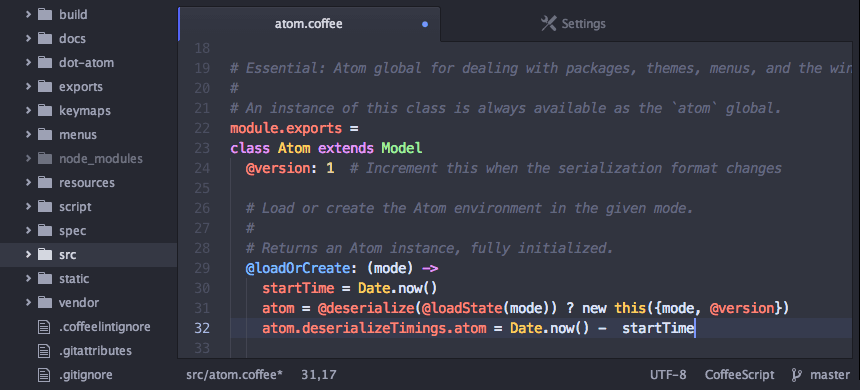
\includegraphics[width=12cm]{figs/atom.png}

\vspace{0.3cm}

  {\Large
    \url{http://atom.io} (Hay paquete Debian)
  }
  
\end{frame}

%%-----------------------------------------------------
\begin{frame}
\frametitle{Características}

\begin{itemize}
  \item Basado HTML, JavaScript, CSS, and Node.js 
  \item Programado en CoffeeScript (compilado a JavaScript)
  \item Autocompletado
  \item Paquetes adicionales
  \item Muchos temas
  \item Configurable
  \item Multiplataforma
  \item ... y es software libre
\end{itemize}

\end{frame}






